\documentclass{article}

\usepackage{graphicx}
\usepackage{tikz}
\usepackage{tikzsymbols}
\usetikzlibrary{calc,patterns,shapes.geometric}
\pagestyle{empty}
\usepackage[margin=0pt]{geometry}
\geometry{papersize={14in,12in}}

\def\centerarc[#1](#2)(#3:#4:#5){\draw[#1] ($(#2)+({#5*cos(#3)},{#5*sin(#3)})$) arc (#3:#4:#5);}

\begin{document}
	\begin{figure}
		\centering
		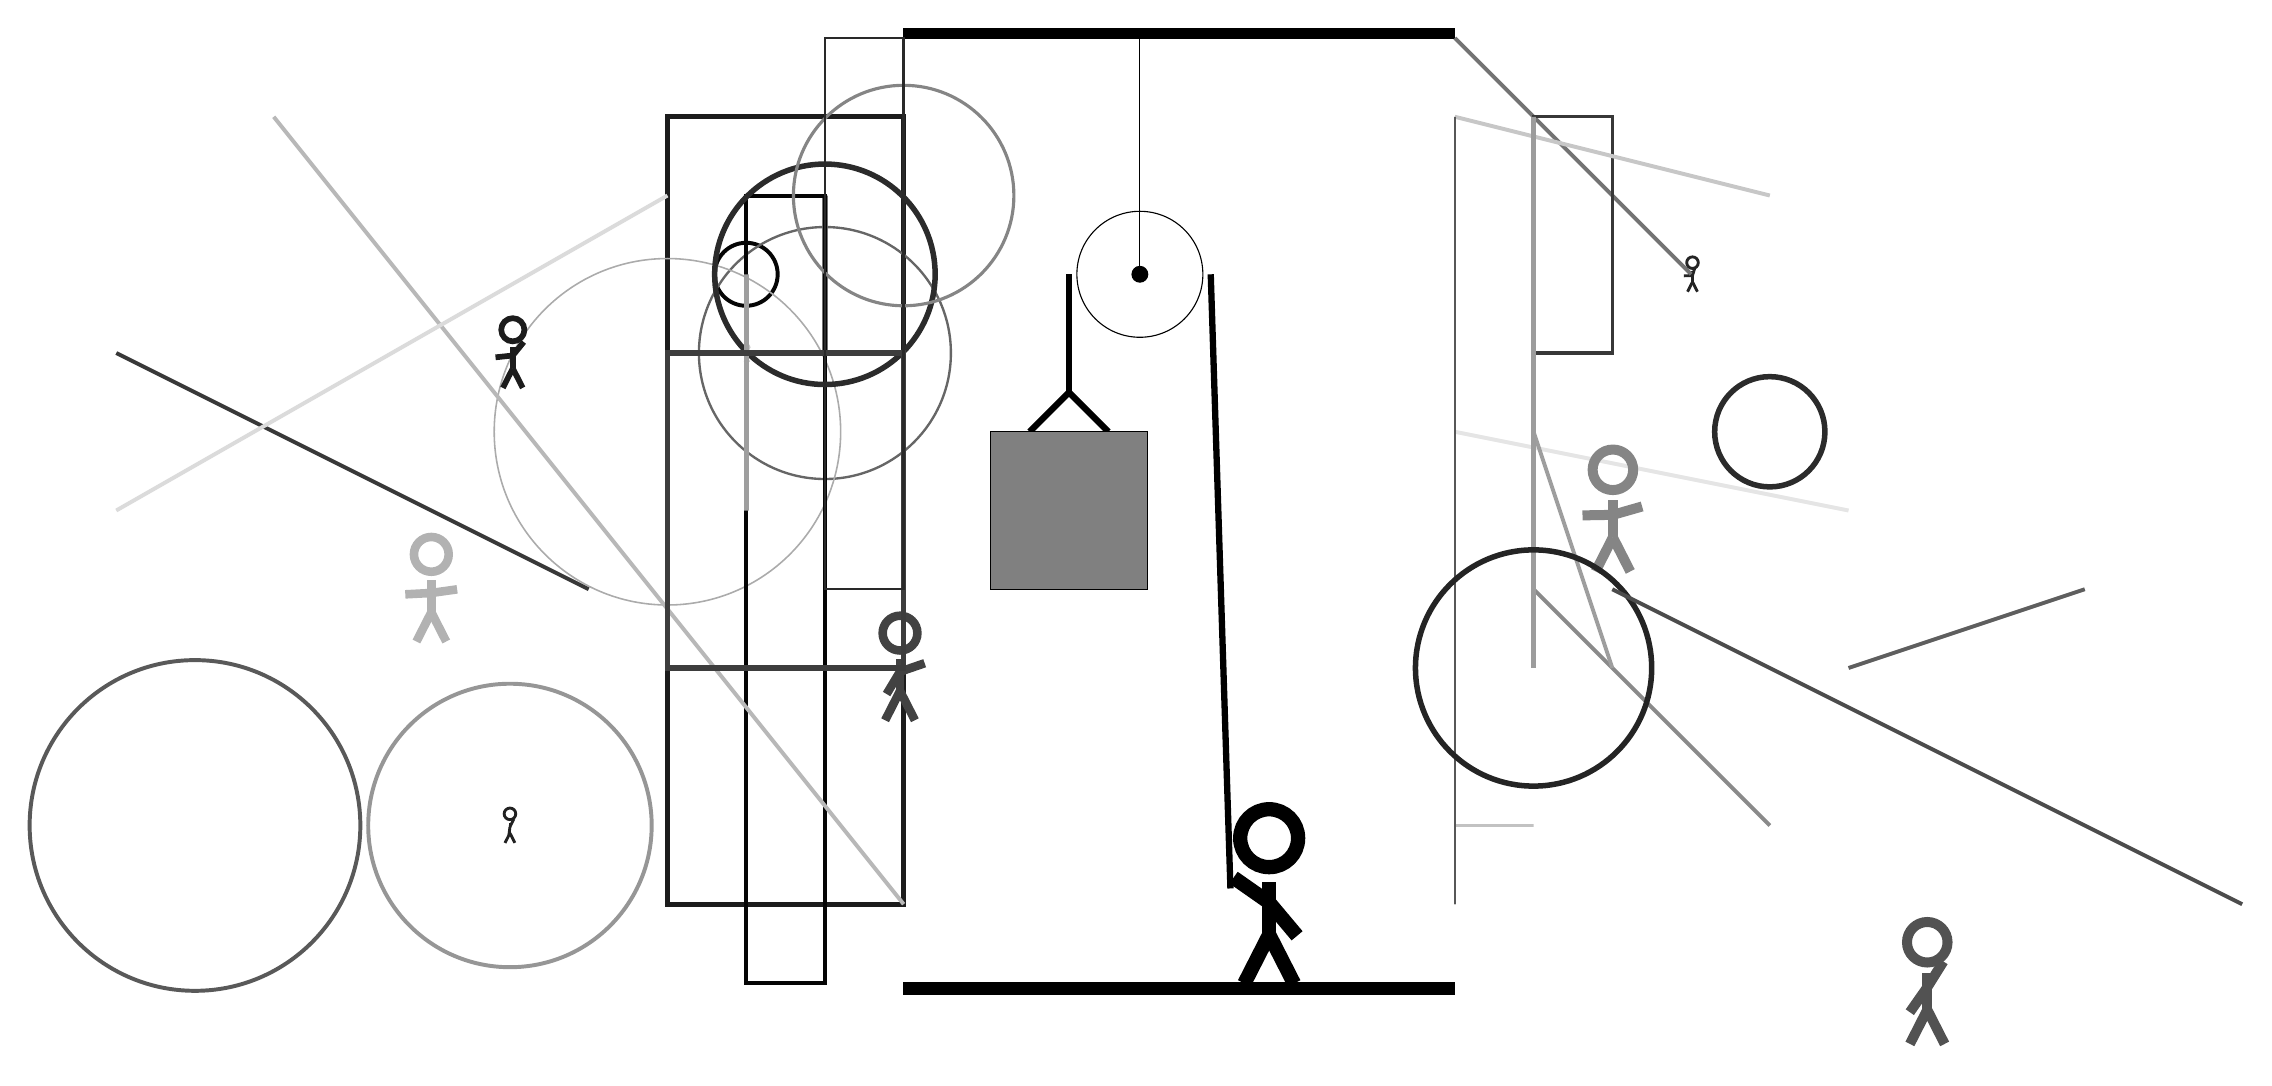
\begin{tikzpicture}
			%%%%% START %%%%%
			
			\draw[fill=black] (-2, 9) rectangle (5, 9.125);
			
			\draw (1, 6) circle (0.8);
			\draw[fill=black] (1, 6) circle (0.1);
			\draw (1, 9) -- (1, 6);
			
			\draw[line width=0.8mm] (-0.4, 4.0) -- (0.1, 4.5) -- (0.6, 4.0);
			\draw[fill=black!50] (-0.9, 4.0) rectangle (1.1, 2.0);
			
			\draw[line width=0.8mm] (0.1, 6) -- (0.1, 4.5);
			\centerarc[line width=0.8mm](1, 6)(0:180:0.9);
			\draw[line width=0.8mm](1.9, 6) -- (2.15, -1.8);
			
			\node[line width=0.6mm, color=black!23] at (-4, 5) {\Strichmaxerl[1][13][80]};
			
			\draw[line width=0.7mm, color=black!55] (-3, 5) rectangle (-3, 7);
			\draw[line width=0.6mm, color=black!89] (-2, 8) rectangle (-5, -2);
			\draw [line width=0.5mm, color=black!98](-4, 6) circle (0.4);
			\draw[line width=0.3mm, color=black!24] (6, -1) rectangle (5, -1);
			\node[line width=0.2mm, color=black!86] at (8, 6) {\Strichmaxerl[2][2][73]};
			\draw [line width=0.3mm, color=black!60](-3, 5) circle (1.6);
			\draw[line width=0.5mm, color=black!10](10, 3) -- (5, 4);
			\draw[line width=0.5mm, color=black!55](8, 6) -- (5, 9);
			\draw[line width=0.3mm, color=black!93] (5, -2) rectangle (5, 3);
			\draw[line width=0.5mm, color=black!46](6, 2) -- (9, -1);
			\draw[line width=0.4mm, color=black!78] (6, 5) rectangle (7, 8);
			\node[line width=0.5mm, color=black!74] at (-2, 1) {\Strichmaxerl[6][59][19]};
			\draw [line width=0.7mm, color=black!83](9, 4) circle (0.7);
			\draw[line width=0.5mm, color=black!78](-6, 2) -- (-12, 5);
			\draw [line width=0.2mm, color=black!33](-5, 4) circle (2.2);
			
			\node[line width=0.7mm, color=black!87] at (-7, -1) {\Strichmaxerl[2][83][63]};
			\draw[line width=0.5mm, color=black!98] (-3, 7) rectangle (-4, -3);
			\draw [line width=0.5mm, color=black!65](-11, -1) circle (2.1);
			
			\draw[line width=0.5mm, color=black!28](-2, -2) -- (-10, 8);
			\draw[line width=0.5mm, color=black!22](9, 7) -- (5, 8);
			\draw [line width=0.7mm, color=black!83](-3, 6) circle (1.4);
			\draw[line width=0.5mm, color=black!38](7, 1) -- (6, 4);
			\draw[line width=0.6mm, color=black!38] (-4, 6) rectangle (-4, 3);
			\draw[line width=0.3mm, color=black!66] (5, 8) rectangle (5, -2);
			\node[line width=0.4mm, color=black!68] at (11, -3) {\Strichmaxerl[7][55][58]};
			
			\draw[line width=0.5mm, color=black!63](10, 1) -- (13, 2);
			\node[line width=0.6mm, color=black!30] at (-8, 2) {\Strichmaxerl[6][3][8]};
			\node[line width=0.2mm, color=black!48] at (7, 3) {\Strichmaxerl[7][1][16]};
			\draw[line width=0.7mm, color=black!39] (6, 1) rectangle (6, 8);
			\draw[line width=0.5mm, color=black!14](-5, 7) -- (-12, 3);
			\draw [line width=0.4mm, color=black!48](-2, 7) circle (1.4);
			\draw[line width=0.7mm, color=black!76] (-2, 5) rectangle (-5, 1);
			\draw [line width=0.5mm, color=black!41](-7, -1) circle (1.8);
			\draw[line width=0.3mm, color=black!84] (-2, 2) rectangle (-3, 9);
			\draw [line width=0.7mm, color=black!86](6, 1) circle (1.5);
			
			\draw[line width=0.5mm, color=black!70](7, 2) -- (15, -2);
			\node[line width=0.3mm, color=black!89] at (-7, 5) {\Strichmaxerl[4][6][51]};
			
			\node at (2.6, -1.9) {\Strichmaxerl[10][-35][-50]};
			
			\draw[fill=black] (-2, -3) rectangle (5, -3.15);
			
			%%%%% END %%%%%
		\end{tikzpicture}
	\end{figure}	
\end{document}